\section{NODE SOFTWARE}

\subsection{Description of the implementation}

The system extends the functionality of the Mbed-OS \acrshort{lorawan} example provided by the teachers, in which an event-queue is provided.

ThIS event-queue provides an asynchronous event dispatcher, in this case for \acrshort{lorawan} events. And, for any event that happens in the system, a callback will be done to process that situation. This working can be seen in the next figure.

\begin{figure}[H]
    \centering
    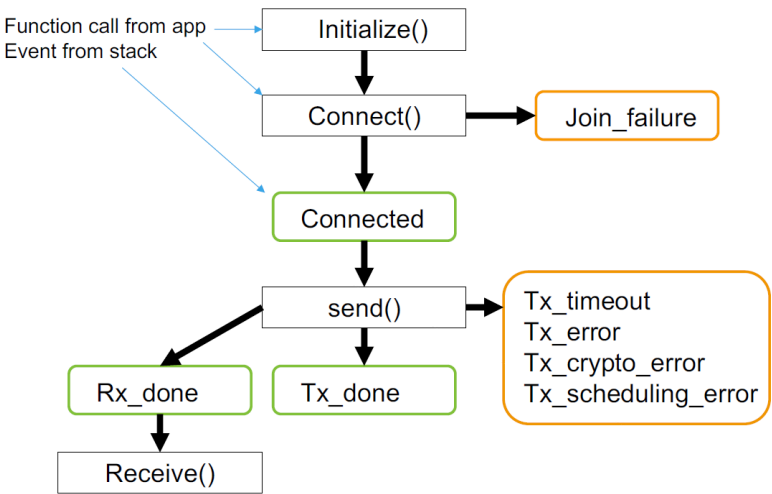
\includegraphics[width=0.6\textwidth]{images/4/event-queue.png}
    \caption{EventQueue process\cite{SensorNetworksProject1_slides_2024}}
    \label{fig:events}
\end{figure}

The solution is implemented by extending the previous event-queue. This event queue will detect possible TX windows in the \acrshort{lorawan} PHY layer and create an event to send a new message with data regarding the measurements of the plant sensors. These sensors are: 
GPS, brightness, soil moisture, humidity, temperature, linear acceleration, RGB data and led status.

To obtain this data, measurement threads are changed from the previous project, these threads read new values each 5 seconds and store the data in an mutex-controlled structure. This structure is later used when the \acrshort{lorawan} stack detects a possible transmitting window.

The threads defined for the solution are:
\begin{itemize}
    \item Main thread with the event-queue.
    \item I2C thread.
    \item GPS thread.
\end{itemize}
\subsection{Modules}
The modules used for this project are mainly the same from the previous course project, with the only exception being a new module to allocate the shared data for the communication between threads.

The module are also used by the same threads:
\begin{itemize}
    \item The I2C thread communicates with the accelerometer, temperature \& humidity and the color module.
    \item The GPS thread controls only the GPS module.
\end{itemize}

\clearpage
\subsection{Threads and communication design} % Comentar los cambios realizados

As we are using \acrshort{lorawan}, which analyzes a possible transmitting window for the next message, we need a method that ensures the maximum utilization of these windows without depending on the main thread. The final design for this can be seen in the next figure.

\begin{figure}[H]
    \centering
    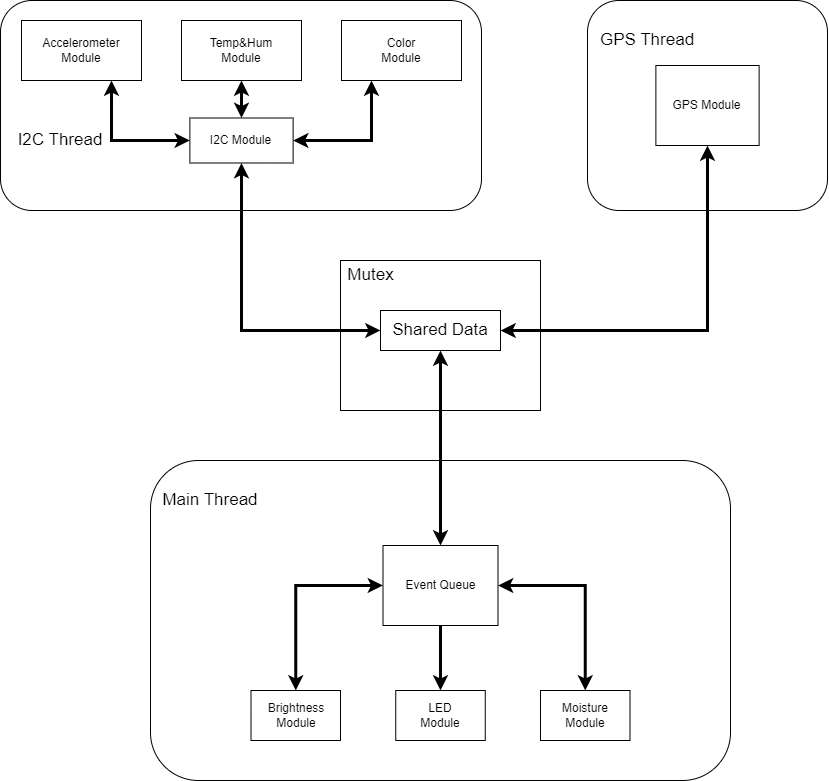
\includegraphics[width=0.8\textwidth]{images/4/Modules.png}
    \caption{Final module design for the system}
    \label{fig:modules}
\end{figure}
%TODO QUITAR LOS "WE"
In the previous project, the approach was having the main thread controlling the execution of the measuring threads with signals. In this project, that won't work because the main thread is controlled by the event-queue. 
To solve this and taking into account the best-effort nature of the system, the decision was to make the measuring threads run independently of the main thread, waking themself up every \texttt{N} seconds. 

The communication between the measuring threads and the main thread had to be redone as well, as in the previous project used an intermediate queue. In this system that could create problems in the next events:
\begin{itemize}
    \item The system doesn't control the time between readings of the data, so there's a possibility of filling of the queue.
    \item The system only focuses on sending the last measurements possible for each sensor, so there's no need for previous data that isn't processed.
\end{itemize}

To solve all this situation, the communication was reduced to a shared structure that contains all the necessary data that is going to be sent through \acrshort{lorawan}. The access to this common structure is done using a Mbed-OS mutex, that ensures the protection of the data and only allows the access of one thread at a time.

This structure is designed to be directly sent to the \acrshort{lorawan} software stack, so it's designed as a network frame. The structure is presented in the \hyperref[appendix]{appendix} and it's explained in the next chapters.
\subsection{Frame design}